\subsection{Поиск неподвижных точек}

\begin{definition}
    Пусть задано отображение $f:\R\rightarrow\R$. Неподвижной точкой системы $u_{t+1} = f(u_t)$ называется точка $u^*$ такая, что $u^* = f(u^*)$. \cite[стр.~82]{bratus10}
\end{definition}

Для системы \ref{eq:first_discrete_system} отображение $f$ имеет вид $f(u)=r u^2 e^{-u}$. Поэтому неподвижными точками системы \ref{eq:first_discrete_system} будут решения уравнения
\begin{equation}\label{OneStepFind}
        u^* = r (u^*)^2 e^{-u^*}.
\end{equation}
Найдем его корни:
$$
    r(u^*)^2e^{-u^*} - u^* = 0
    \;
    \Longleftrightarrow
    \;
    u^* (r u^* e^{-u^*} - 1) = 0
    \;
    \Longleftrightarrow
    \;
    \left[
    \begin{gathered}
        u^* = 0 \\
        u^* e^{-u^*} = \frac{1}{r}
    \end{gathered}
    \right.
$$
Найдем решения второго уравнения получившейся совокупности.
\begin{equation}\label{eq:fix_point_equation}
    u^* e^{-u^*} = \frac{1}{r}
\end{equation}
Для этого рассмотрим левую часть равенства 
$$
    g(u) = u e^{-u}.
$$
    Функция $g(u)$ --- непрерывно дифференцируема в $\R_+$ и имеет производную
$$
    g'(u) = e^{-u} - u e^{-u} = e^{-u} (1 - u).
$$
Производная $g'(u)$ принимает положительные значения при $u \in (-\infty, 1)$, отрицательные значения --- при $u \in (1, +\infty)$ и равна нулю при $u = 1$. Из этого следует, что $u = 1$ --- точка глобального максимума функции $g(u)$. $g(1) = \frac{1}{e}$. (Рис.~\ref{img:helped_function_g})



Получается, что уравнение \ref{eq:fix_point_equation} при $0 < r < e$ не имеет решений; при $r = e$ имеет единственное решение $u^* = 1$ и при $r > 0$ имеет два корня $u^*_1$ и $u^*_2$, причем $u^*_1 \in (0, 1)$, а $u^*_2 \in (1, +\infty)$. В последнем случае посчитать решения аналитически не представляется возможным. (Рис.~\ref{img:one_step_system_solve_fix})


            
Подведем итог. Система \ref{eq:first_discrete_system} в зависимости от параметра $r$ имеет следующие неподвижные точки:
\begin{enumerate}
    \item $0 < r < e$:
    $$
        u^* = 0.
    $$
    \item $r = e$:
    $$
        u^*_1 = 0, \; u^*_2 = 1.
    $$
    \item $r > e$:
    $$
        u^*_1 = 0, \; u^*_2 \in (0, 1), \; u^*_3 \in (1, +\infty).
    $$
\end{enumerate}

\begin{figure}[h]
        \centering
        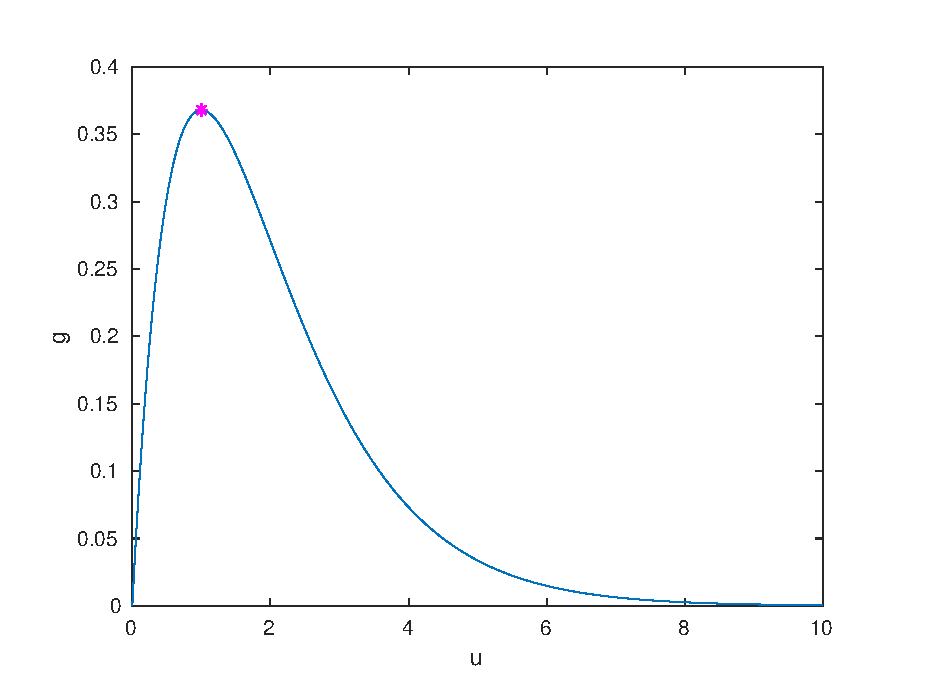
\includegraphics[width=0.8\linewidth]{first_discrete_system/searching_of_fixed_points/g.eps}
        \caption{Поведение функции $g(u)$ на рассматриваемом промежутке}
        \label{img:helped_function_g}
\end{figure}

\begin{figure}[h]
        \centering
        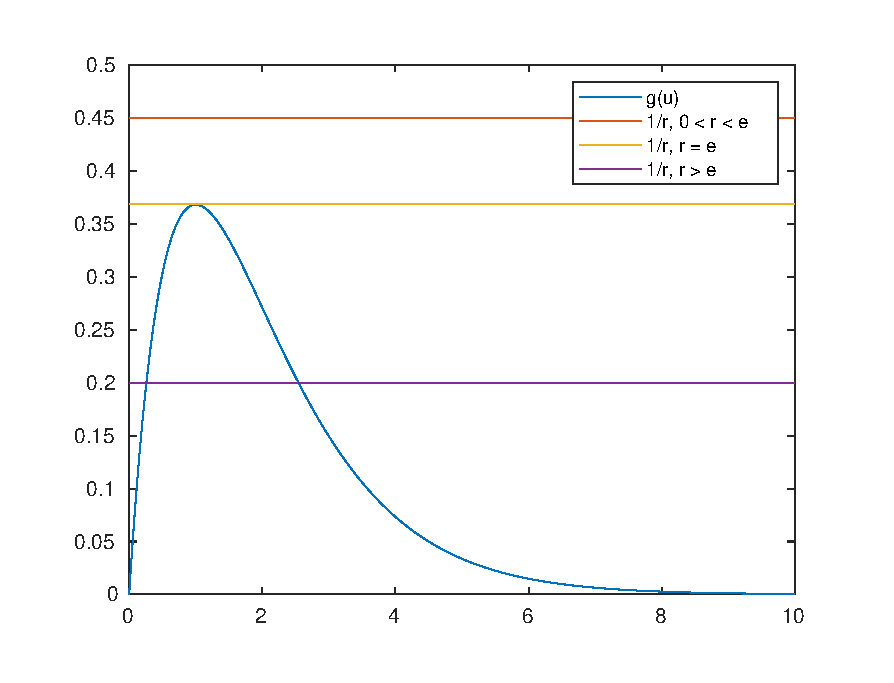
\includegraphics[width=0.8\linewidth]{first_discrete_system/searching_of_fixed_points/roots.eps}
        \caption{Количество корней уравнения $u^* e^{-u^*} = \frac{1}{r}$}
        \label{img:one_step_system_solve_fix}
\end{figure}

\clearpage